\input{../utils/preamble}
\createdgmtitle{supp}
%--------------------------------------------------------------------------------
\begin{document}
%--------------------------------------------------------------------------------
\begin{frame}
%\thispagestyle{empty}
\titlepage
\end{frame}
%=======
\begin{frame}{IWAE, 2015}
How to determine whether all VAE latent variables are informative?
\[
A_{i} = \text{cov}_\bx \left( \mathbb{E}_{q(z_i | \bx)} [z_i] \right) > 0.01 \quad \Leftrightarrow \quad z_i \text{ is active}
\]
\begin{figure}
	\centering
	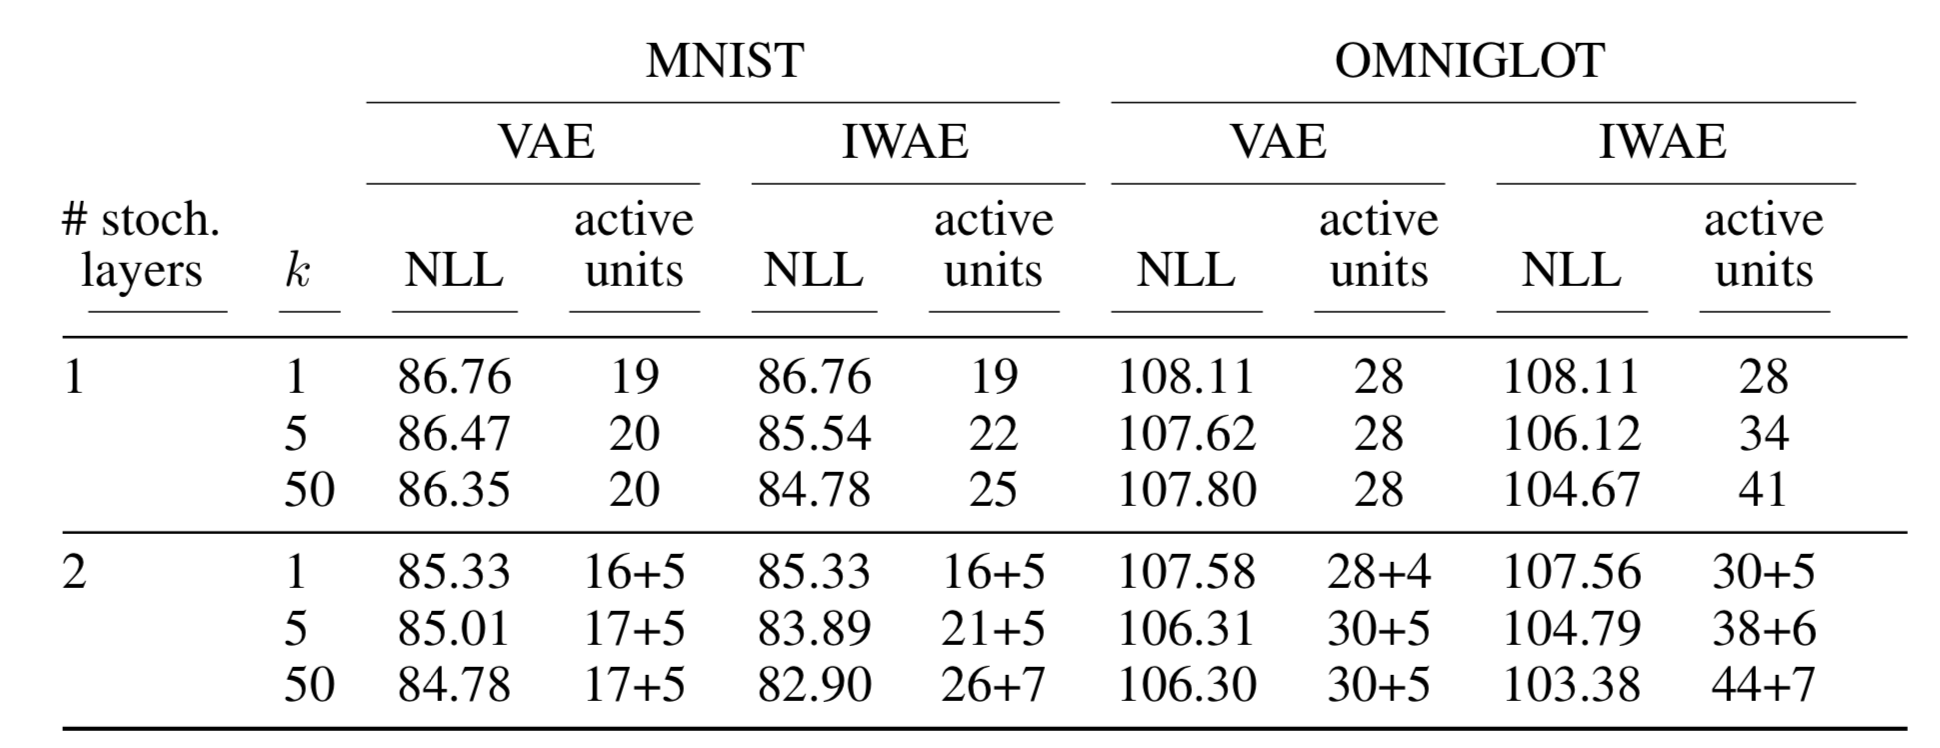
\includegraphics[width=\linewidth]{figs/IWAE_3.png}
\end{figure}
\vfill
\hrule\medskip
{\scriptsize \href{https://arxiv.org/pdf/1509.00519.pdf}{https://arxiv.org/pdf/1509.00519.pdf}}
\end{frame}
%=======
 \begin{frame}{GatedPixelCNN (2016)}
 \begin{figure}
     \centering
     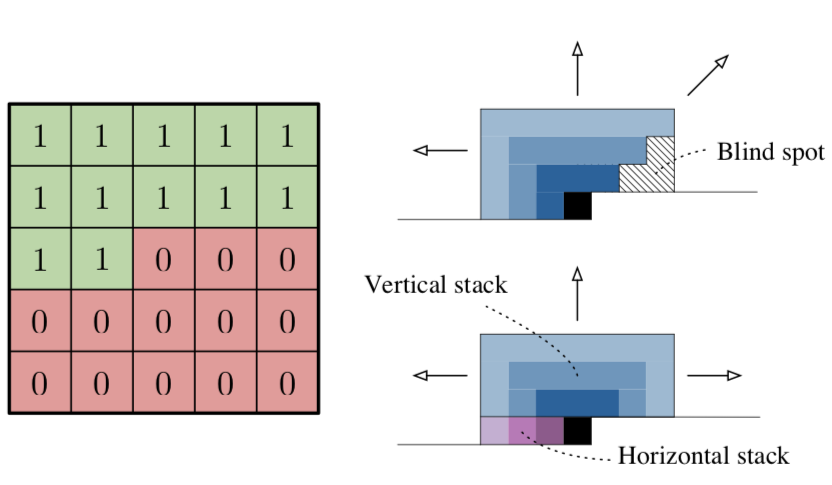
\includegraphics[width=0.5\linewidth]{figs/gatedpixelcnn.png}
     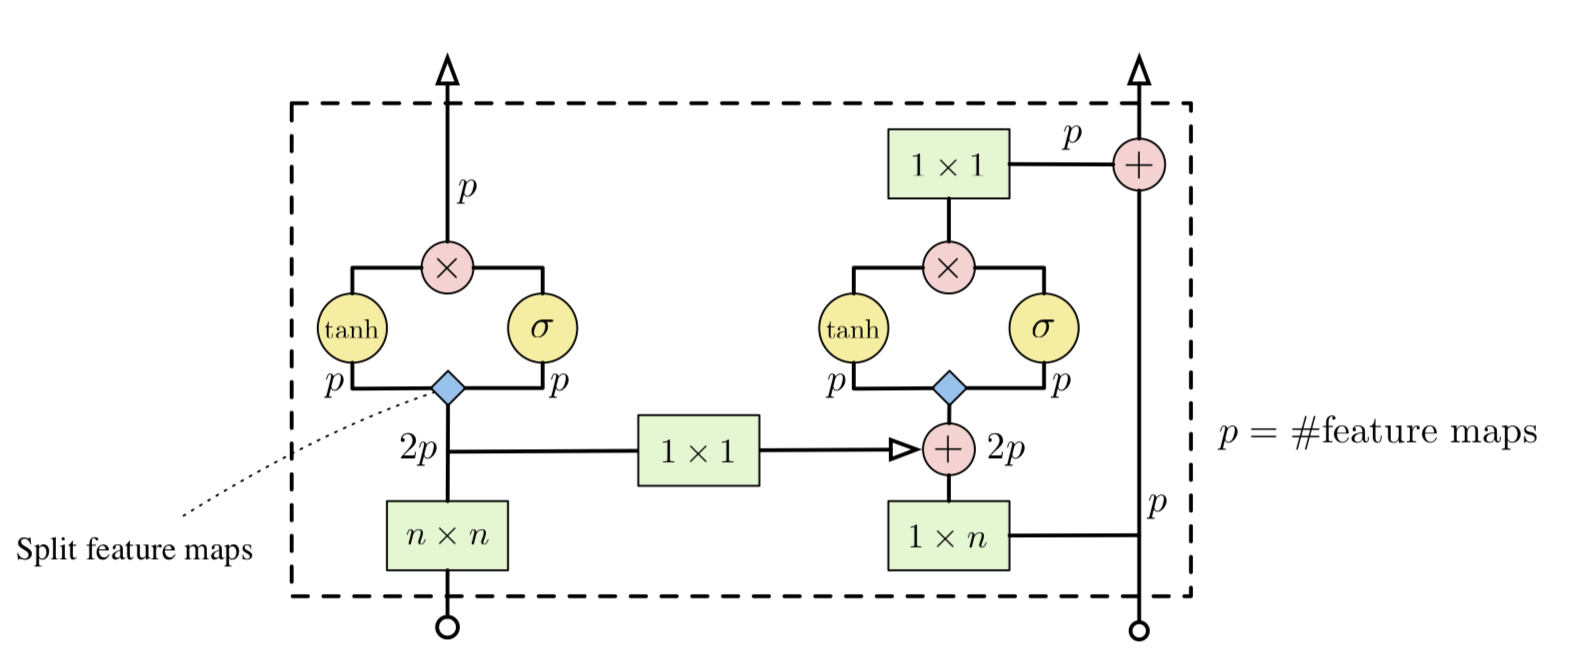
\includegraphics[width=0.5\linewidth]{figs/gated_block.png}
 \end{figure}
 \vfill
 \hrule\medskip
 {\scriptsize Van den Oord A. et al. Conditional image generation with pixelcnn decoders \href{https://arxiv.org/pdf/1606.05328.pdf}{https://arxiv.org/pdf/1606.05328.pdf}}
 \end{frame}
 %=======
 \begin{frame}{GatedPixelCNN (2016)}
 \begin{minipage}[t]{0.5\columnwidth}
 	\begin{figure}[h]
 		\centering
 		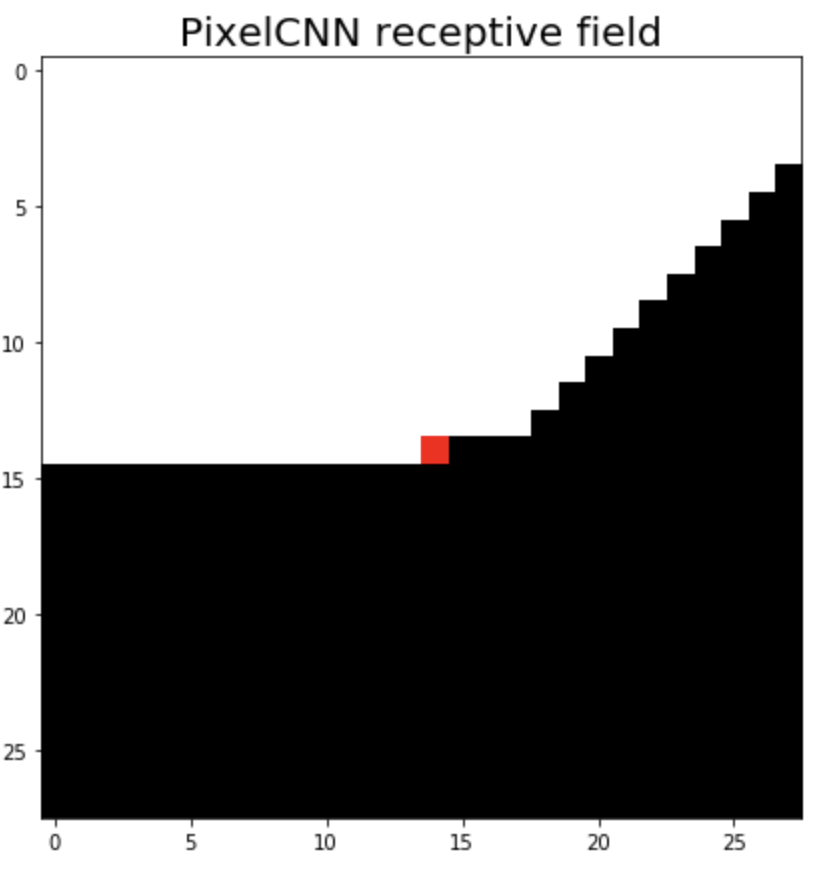
\includegraphics[width=0.9\linewidth]{figs/pixelcnn_receptive_field.png}
 	\end{figure}
 \end{minipage}%
 \begin{minipage}[t]{0.5\columnwidth}
 	\begin{figure}[h]
 		\centering
 		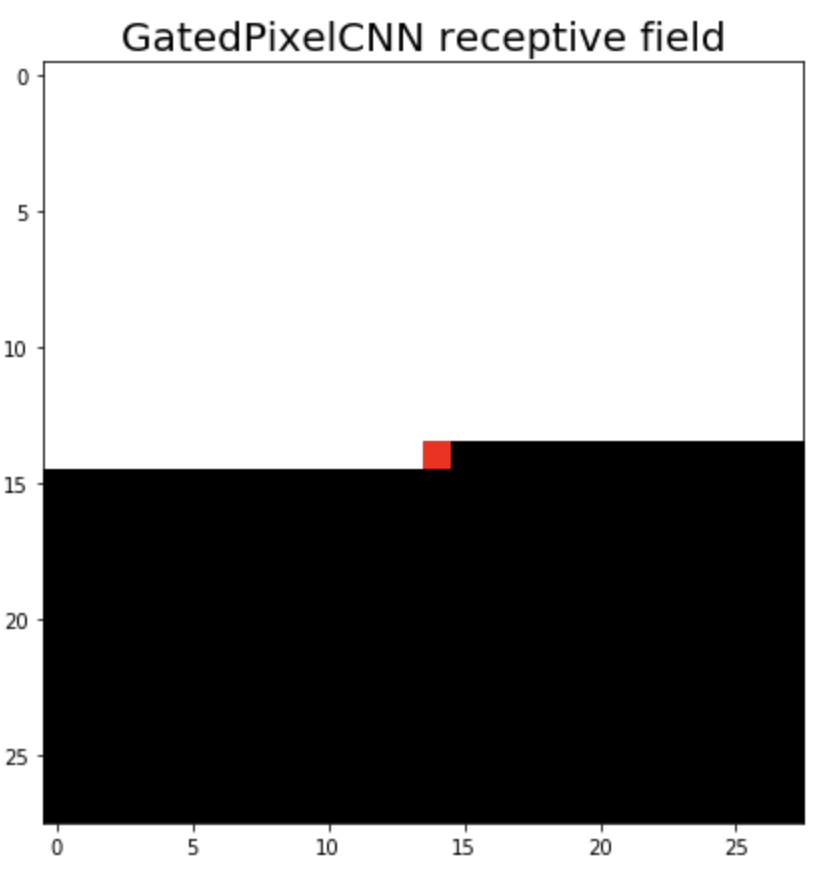
\includegraphics[width=0.9\linewidth]{figs/gatedpixelcnn_receptive_field.png}
 	\end{figure}
 \end{minipage}
 \vfill
 \hrule\medskip
 {\scriptsize Van den Oord A. et al. Conditional image generation with pixelcnn decoders \href{https://arxiv.org/pdf/1606.05328.pdf}{https://arxiv.org/pdf/1606.05328.pdf}}
 \end{frame}
 %=======
 \begin{frame}{Extensions}
     \begin{itemize}
         \item \textbf{PixelCNN++}: \textit{Improving the PixelCNN with Discretized Logistic Mixture Likelihood and Other Modifications} \\
         \href{https://arxiv.org/pdf/1701.05517.pdf}{https://arxiv.org/pdf/1701.05517.pdf} \\
         (mixture of logistics instead of softmax);
         \item \textbf{PixelSNAIL}: \textit{An Improved Autoregressive Generative Model} \\
         \href{https://arxiv.org/pdf/1712.09763.pdf}{https://arxiv.org/pdf/1712.09763.pdf} \\
         (self-attention to learn optimal autoregression ordering).
     \end{itemize}
 \end{frame}
%=======
\begin{frame}{PixelVAE, 2016}
	\begin{block}{Hierarchical VAE}
		\begin{figure}
			\centering
			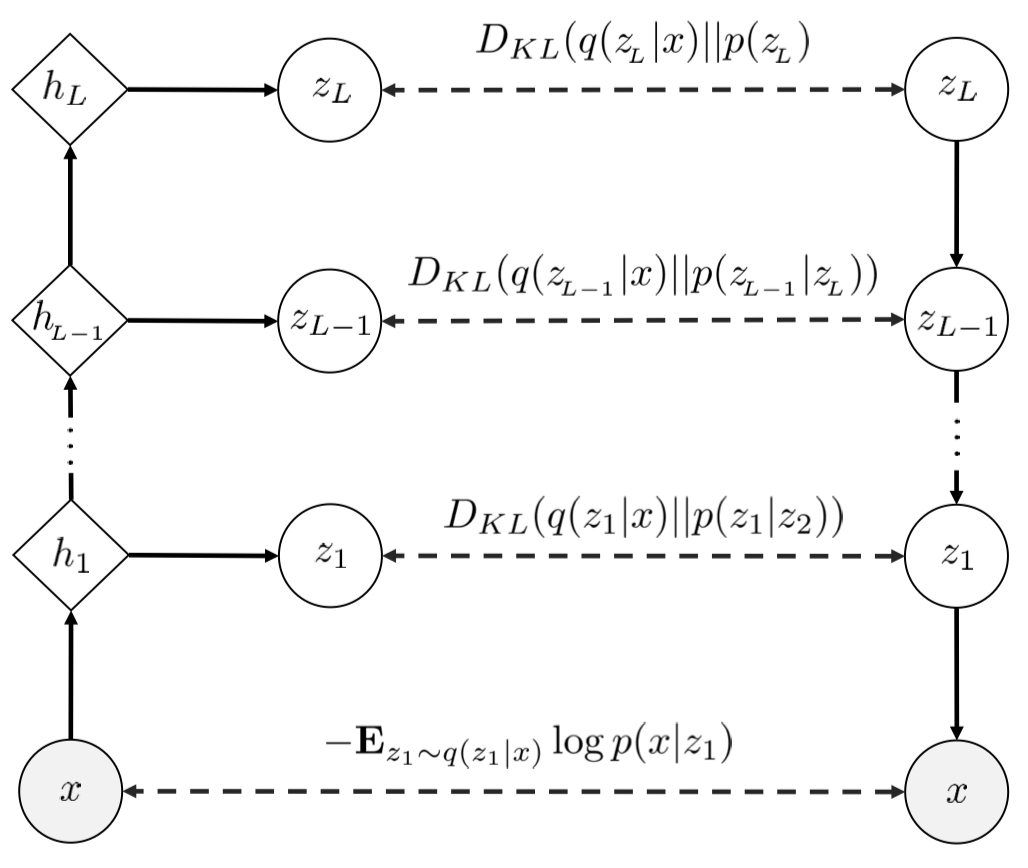
\includegraphics[width=0.7\linewidth]{figs/PixelVAE_1.png}
		\end{figure}
	\end{block}
	\vfill
	\hrule\medskip
	{\scriptsize \href{https://arxiv.org/pdf/1611.05013.pdf}{https://arxiv.org/pdf/1611.05013.pdf}}
\end{frame}
%=======
\begin{frame}{PixelVAE, 2016}
	\begin{block}{Hierarchical decomposition}
		\vspace{-1cm}
		\begin{align*}
			p(\bz_1, \dots, \bz_L) &= p(\bz_L) p(\bz_{L-1} | \bz_L) \dots p(\bz_1, \bz_2); \\
			q(\bz_1, \dots, \bz_L | \bx) &= q(\bz_1 | \bx) \dots q(\bz_L | \bx).
		\end{align*}
	\end{block}
	\vspace{-0.5cm}
	\begin{block}{ELBO}
		\vspace{-0.5cm}
		{\footnotesize
			\begin{align*}
				\mathcal{L}(q, \btheta) &= \mathbb{E}_{q(\bz_1 | \bx)} \log p(\bx | \bz_1, \btheta) - KL(q(\bz_1, \dots, \bz_L | \bx) || p(\bz_1, \dots, \bz_L)) \\
				&= \mathbb{E}_{q(\bz_1 | \bx)} \log p(\bx | \bz_1, \btheta) - \int \prod_{j=1}^L q(\bz_j | \bx) \sum_{i=1}^L \log \frac{q(\bz_i | \bx)}{p(\bz_i | \bz_{i + 1})} d \bz_1 \dots d \bz_L \\
				&= \mathbb{E}_{q(\bz_1 | \bx)} \log p(\bx | \bz_1, \btheta) - \sum_{i=1}^L \int \prod_{j=1}^L q(\bz_j | \bx) \log \frac{q(\bz_i | \bx)}{p(\bz_i | \bz_{i + 1})} d \bz_1 \dots d \bz_L \\
				&= \mathbb{E}_{q(\bz_1 | \bx)} \log p(\bx | \bz_1, \btheta) - \sum_{i=1}^L \int q(\bz_{i+1} | \bx) q(\bz_i | \bx) \log \frac{q(\bz_i | \bx)}{p(\bz_i | \bz_{i + 1})} d \bz_i d \bz_{i+1} \\
				&= \mathbb{E}_{q(\bz_1 | \bx)} \log p(\bx | \bz_1, \btheta) - \sum_{i=1}^L \mathbb{E}_{q(\bz_{i+1} | \bx)} \left[ KL (q(\bz_i | \bx) || p(\bz_i | \bz_{i + 1}))\right]
			\end{align*}
		}
	\end{block}
	\vfill
	\hrule\medskip
	{\scriptsize \href{https://arxiv.org/pdf/1611.05013.pdf}{https://arxiv.org/pdf/1611.05013.pdf}}
\end{frame}%=======
\begin{frame}{RevNets, 2017}
	\begin{minipage}[t]{0.6\columnwidth}
		\begin{itemize}
			\item Modern neural networks are trained via backpropagation.
			\item Residual networks are state of the art in image classification.
			\item Backpropagation requires storing the network activations.
		\end{itemize}
	\end{minipage}%
	\begin{minipage}[t]{0.4\columnwidth}
		\begin{figure}
			\centering
			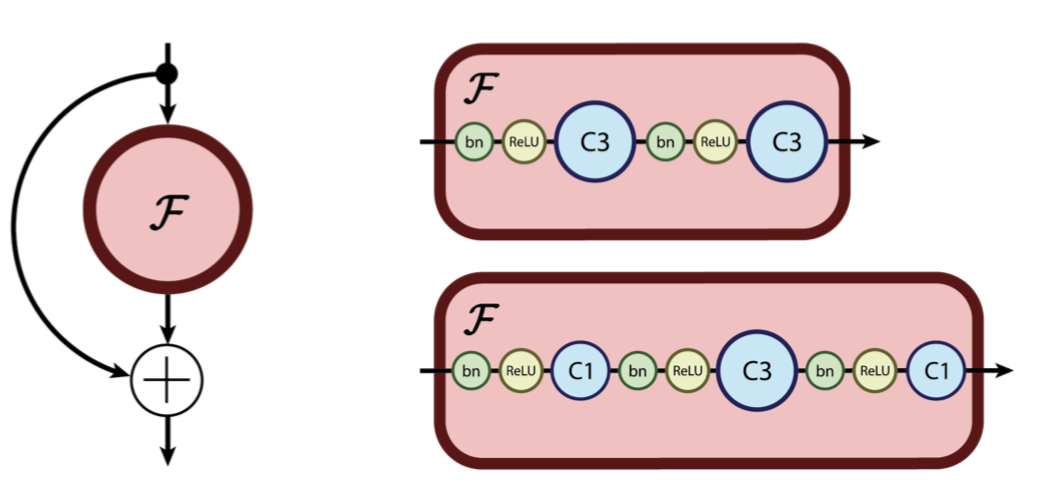
\includegraphics[width=\linewidth]{figs/resnet_block.png}
		\end{figure}
	\end{minipage}
	\vspace{0.1cm}
	\begin{block}{Problem}
		Storing the activations imposes an increasing memory burden. GPUs have limited memory capacity, leading to constraints often exceeded by state-of-the-art architectures (with thousand layers).
	\end{block}
	\myfootnotewithlink{https://arxiv.org/abs/1707.04585}{Gomez A. N. et al. The Reversible Residual Network: Backpropagation Without Storing Activations, 2017}
\end{frame}
%=======
\begin{frame}{RevNets, 2017}
	\begin{block}{NICE}
		\vspace{-0.2cm}
		\begin{equation*}
			\begin{cases} \bz_1 = \bx_1; \\ \bz_2 = \bx_2 + \mathcal{F}(\bx_1, \btheta);\end{cases}  \quad \Leftrightarrow \quad 
			\begin{cases} \bx_1 = \bz_1; \\ \bx_2 = \bz_2 - \mathcal{F}(\bz_1, \btheta).\end{cases} 
		\end{equation*}
		\vspace{-0.2cm}
	\end{block}
	\begin{block}{RevNet}
		\begin{equation*}
			\begin{cases} \by_1 = \bx_1 + \mathcal{F}(\bx_2, \btheta); \\ \by_2 = \bx_2 + \mathcal{G}(\by_1, \btheta);\end{cases} \quad \Leftrightarrow \quad 
			\begin{cases} \bx_2 = \by_2 - \mathcal{F}(\by_1, \btheta); \\ \bx_1 = \by_1 - \mathcal{G}(\bx_2, \btheta).\end{cases} 
		\end{equation*}
	\end{block}
	\begin{figure}
		\centering
		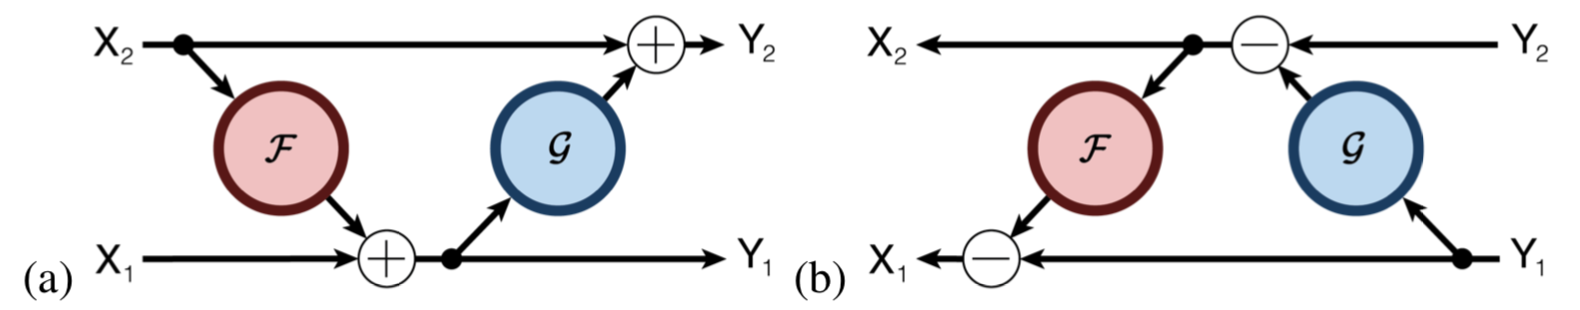
\includegraphics[width=\linewidth]{figs/revnet.png}
	\end{figure}
	\myfootnotewithlink{https://arxiv.org/abs/1707.04585}{Gomez A. N. et al. The Reversible Residual Network: Backpropagation Without Storing Activations, 2017}
\end{frame}
%=======
\begin{frame}{RevNets, 2017}
	\begin{figure}
		\centering
		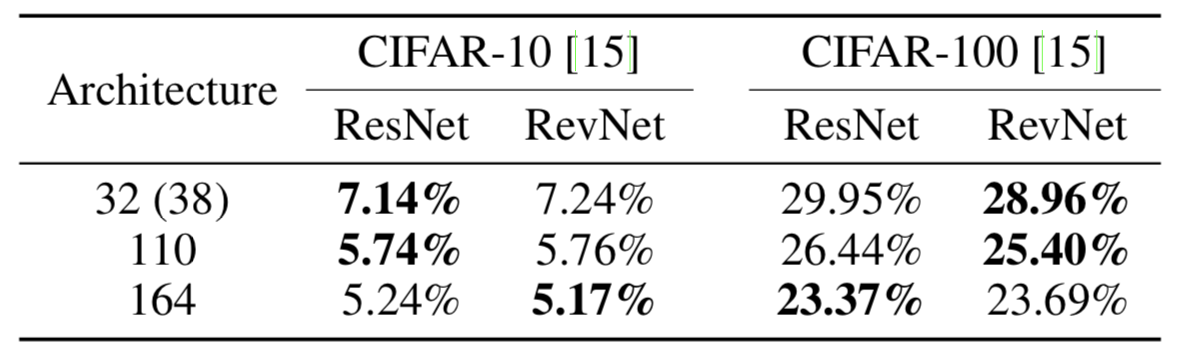
\includegraphics[width=0.8\linewidth]{figs/revnet_results.png}
	\end{figure}
	\begin{itemize}
		\item If the network contains non-reversible blocks (poolings, strides), activations for these blocks should be stored.
		\item To avoid storing activations in the modern frameworks, the backward pass should be manually redefined.
	\end{itemize}
	\myfootnotewithlink{https://arxiv.org/abs/1707.04585}{Gomez A. N. et al. The Reversible Residual Network: Backpropagation Without Storing Activations, 2017}
\end{frame}
%=======
\begin{frame}{i-RevNet, 2018}
	\begin{block}{Hypothesis}
		The success of deep convolutional networks is based on progressively discarding uninformative variability about the input with respect to the problem at hand. 
	\end{block}
	\begin{itemize}
		\item It is difficult to recover images from their hidden representations. 
		\item Information bottleneck principle: an optimal representation must reduce the MI between an input and its representation to reduce uninformative variability + maximize the MI between the output and its representation to preserve each class from collapsing onto other classes.
	\end{itemize}
	\myfootnotewithlink{https://arxiv.org/abs/1802.07088}{Jacobsen J. H., Smeulders A., Oyallon E. i-RevNet: Deep Invertible Networks, 2018}
\end{frame}
%=======
\begin{frame}{i-RevNet, 2018}
	\begin{block}{Hypothesis}
		The success of deep convolutional networks is based on progressively discarding uninformative variability about the input with respect to the problem at hand. 
	\end{block}
	
	\begin{block}{Idea}
		Build a cascade of homeomorphic layers (i-RevNet), a network that can be fully inverted up to the final projection onto the classes, i.e. no information is discarded.
	\end{block}
	\myfootnotewithlink{https://arxiv.org/abs/1802.07088}{Jacobsen J. H., Smeulders A., Oyallon E. i-RevNet: Deep Invertible Networks, 2018}
\end{frame}
%=======
\begin{frame}{i-RevNet, 2018}
	
	\begin{figure}
		\centering
		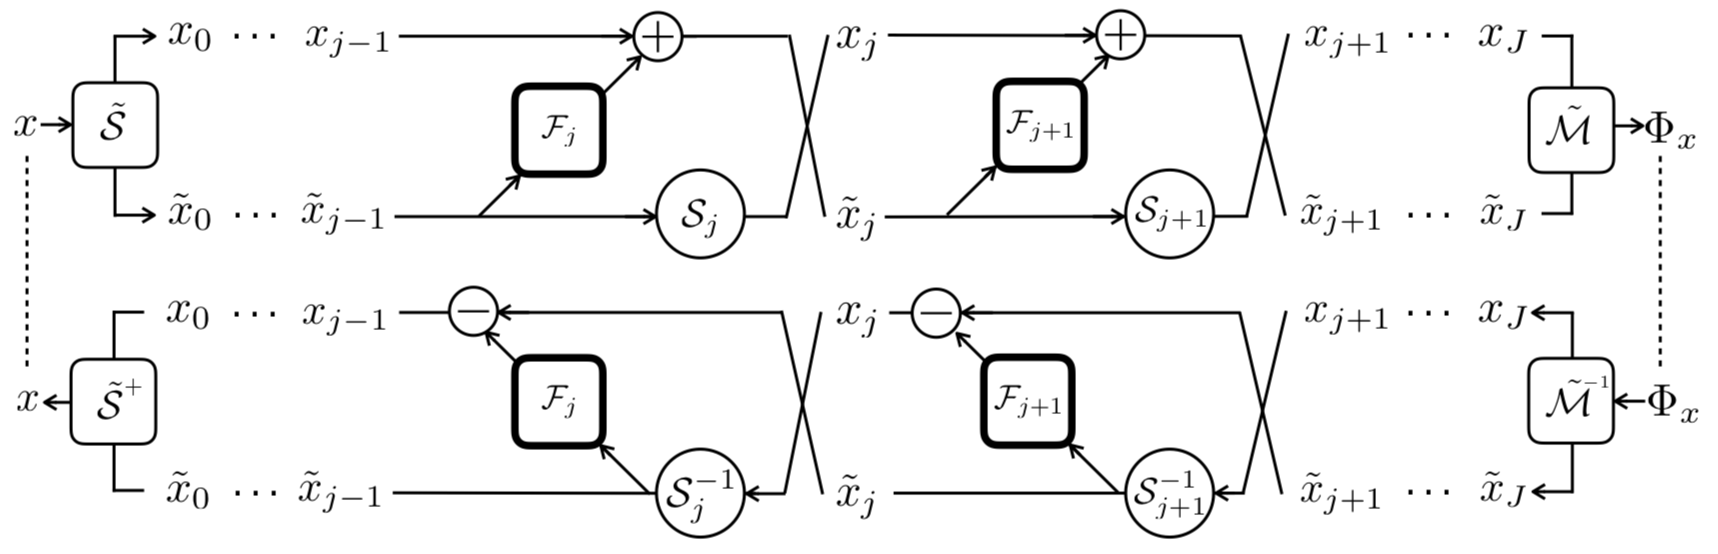
\includegraphics[width=\linewidth]{figs/i-revnet.png}
	\end{figure}
	
	\begin{figure}
		\centering
		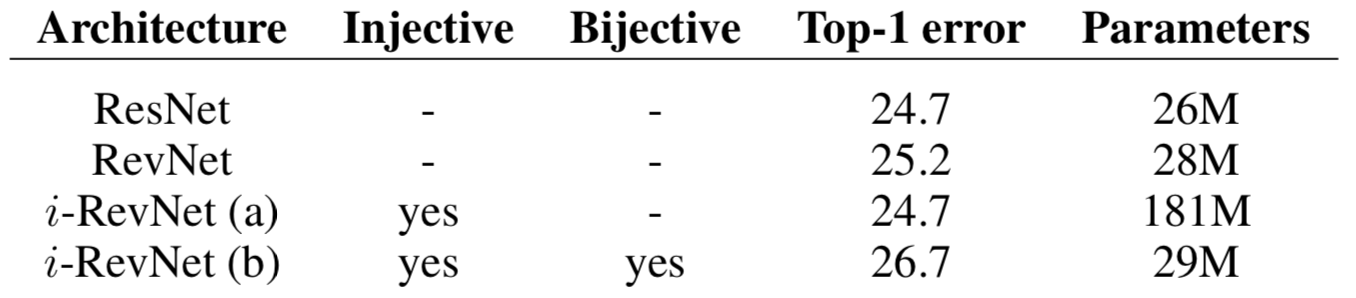
\includegraphics[width=0.9\linewidth]{figs/i-revnet_block.png}
	\end{figure}

	\myfootnotewithlink{https://arxiv.org/abs/1802.07088}{Jacobsen J. H., Smeulders A., Oyallon E. i-RevNet: Deep Invertible Networks, 2018}
\end{frame}

\end{document} 